\section{Visão Geral da Transcodificação Rápida de Vídeo}
\label{cap:3.1}

Os 34 artigos selecionados após as etapas de filtragem estão resumidos na Tabela \ref{tab:III}, apresentando os formatos de decodificação e de codificação utilizados, assim como as métricas BD-rate e TS para cada solução proposta. Todos eles fazem uso de heurísticas para acelerar o transcodificador, com base em análises estatísticas ou em aprendizado de máquina. Em média, os trabalhos de aceleração da transcodificação de vídeo publicados na última década são capazes de reduzir o tempo do processo de transcodificação à metade (TS médio igual à 50,74\%) em comparação com o transcodificador original correspondente. Observando o desvio padrão da redução do tempo, é seguro afirmar que existe uma grande probabilidade de que soluções de transcodificação rápida ofereçam uma redução de tempo entre 31,51\% e 69,97\%. Já o impacto médio na eficiência de codificação (em termos de BD-rate) é de 4,11\%, e não superior a 6,57\% em média (considerando desvio padrão mais a média), indicando que é esperada alguma perda na eficiência de codificação, desde pequenos a médios valores de BD-rate, ao se executar a transcodificação na metade do tempo de um transcodificador original.

\afterpage{
\clearpage

\begin{landscape}
{\footnotesize
\begin{longtblr}[
    caption = {Resumo dos artigos presentes na revisão sistemática da literatura sobre transcodificação rápida de vídeo, publicados entre os anos de 2011 e 2022.},
    label = {tab:III},
    note{1} = {Valor adaptado da métrica ``número de vezes mais rápido que'' (do inglês, \textit{speed-up}) para percentual TS.}
]{
    colspec = {p{5cm}|p{2.2cm}|p{2.2cm}|p{4cm}|c|c|c},
    rowhead = 1,
    hlines,
    row{even} = {gray9}
}
\hline
\textbf{Autor} & \textbf{Formato de Origem} & \textbf{Formato de Destino} & \textbf{Estágios Envolvidos} & \textbf{BD-rate (\%)} & \textbf{TS (\%)} & \textbf{Razão ($\frac{BD-rate}{TS}$)} \\
\citet{bib:leuven_2011} & H.264/AVC & H.264/AVC & particionamento de blocos, predição intraquadro & 7,33 & 95,73 & 0,077 \\
\citet{bib:wang_2012} & H.264/AVC & H.264/AVC & predição interquadros & 3,53 & 90,62 & 0,039 \\
\citet{bib:aminlou_2016} & H.264/AVC & H.264/AVC & predição interquadros & 6,60 & 6,80 & 0,971 \\
\SetCell[c=4]{r}\textit{Média de H.264/AVC-to-H.264/AVC} &&&& \textit{5.82} & \textit{64.38} & \\
\SetCell[c=4]{r}\textit{Desvio Padrão de H.264/AVC-to-H.264/AVC} &&&& \textit{2,02} & \textit{49,93} & \\

\citet{bib:zhang_2012} & H.264/AVC & H.265/HEVC & particionamento de blocos, predição intraquadro e predição interquadros & 30,00 & 80,00 & 0,375 \\
\citet{bib:peixoto_2012} & H.264/AVC & H.265/HEVC & predição interquadros & 5,49 & 52,74 & 0,104 \\
\citet{bib:jiang_2013} & H.264/AVC & H.265/HEVC & predição interquadros & 1,45 & 30,50 & 0,048 \\
\citet{bib:peixoto_2014} & H.264/AVC & H.265/HEVC & predição interquadros & 3,87 & 63,06 & 0,061 \\
\citet{bib:peixoto2_2014} & H.264/AVC & H.265/HEVC & particionamento de blocos & 8,41 & 70,54 & 0,119 \\
\citet{bib:honrubia_2014} & H.264/AVC & H.265/HEVC & particionamento de blocos & 4,80 & 64,29 & 0,075 \\
\citet{bib:peixoto3_2014} & H.264/AVC & H.265/HEVC & particionamento de blocos, predição intraquadro e predição interquadros & 3,32 & 49,75\TblrNote{1} & 0,067 \\
\citet{bib:nagaraghatta_2015} & H.264/AVC & H.265/HEVC & predição interquadros & 4,20 & 50,33 & 0,083 \\
\citet{bib:franche_2015} & H.264/AVC & H.265/HEVC & BP. predição interquadros & 3,28 & 87,32 & 0,038 \\
\citet{bib:honrubia_2015} & H.264/AVC & H.265/HEVC & particionamento de blocos & 5,20 & 60,00\TblrNote{1} & 0,087 \\
\citet{bib:honrubia_2016} & H.264/AVC & H.265/HEVC & particionamento de blocos & 2,20 & 57,37 & 0,038 \\
\citet{bib:correa_2016} & H.264/AVC & H.265/HEVC & particionamento de blocos & 1,67 & 44,10 & 0,038 \\
\citet{bib:franche_2017} & H.264/AVC & H.265/HEVC & predição interquadros & 10,13 & 67,90 & 0,149 \\
\citet{bib:liu_2018} & H.264/AVC & H.265/HEVC & particionamento de blocos & 1,83 & 53,71 & 0,034 \\
\citet{bib:xu_2019} & H.264/AVC & H.265/HEVC & particionamento de blocos & 1,16 & 59,60 & 0,019 \\
\citet{bib:soares_2019} & H.264/AVC & H.265/HEVC & particionamento de blocos & 0,75 & 24,28 & 0,031 \\
\citet{bib:xin_2022} & H.264/AVC & H.265/HEVC & particionamento de blocos & 0,60 & 38,40 & 0,015 \\
\SetCell[c=4]{r}\textit{Média de H.264/AVC-to-H.265/HEVC} &&&& \textit{5,20} & \textit{56,11} \\
\SetCell[c=4]{r}\textit{Desvio Padrão de H.264/AVC-to-H.265/HEVC} &&&& \textit{2,71} & \textit{15,59} \\

\citet{bib:sung_2014} & H.265/HEVC & H.265/HEVC & particionamento de blocos & 1,46 & 51,02 & 0,029 \\
\citet{bib:nguyen_2015} & H.265/HEVC & H.265/HEVC & particionamento de blocos & 0,88 & 40,50 & 0,022 \\
\citet{bib:grellert_2018} & H.265/HEVC & H.265/HEVC & particionamento de blocos & 0,29 & 41,81 & 0,007 \\
\citet{bib:lindino_2021} & H.265/HEVC & H.265/HEVC & particionamento de blocos & 0,54 & 42,00 & 0,013 \\
\citet{bib:xin_2022} & H.265/HEVC & H.265/HEVC & particionamento de blocos & 0,60 & 38,40 & 0,015 \\
\SetCell[c=4]{r}\textit{Média de H.265/HEVC-to-H.265/HEVC} &&&& \textit{5.20} & \textit{56,11} \\
\SetCell[c=4]{r}\textit{Desvio Padrão de H.265/HEVC-to-H.265/HEVC} &&&& \textit{2,71} & \textit{15,59} \\

\citet{bib:borges_2019} & H.265/HEVC & AV1 & particionamento de blocos & 4,55 & 35,41 & 0,128 \\
\citet{bib:borges2_2019} & H.265/HEVC & AV1 & particionamento de blocos & 4,94 & 35,43 & 0,139 \\
\citet{bib:chen_2019} & H.265/HEVC & AV1 & particionamento de blocos & 0,79 & 37,80 & 0,021 \\
\citet{bib:borges2_2021} & H.265/HEVC & AV1 & particionamento de blocos & 5,38 & 34,06 & 0,158 \\
\SetCell[c=4]{r}\textit{Média de H.265/HEVC-to-AV1} &&&& \textit{3,91} & \textit{35,68} \\
\SetCell[c=4]{r}\textit{Desvio Padrão de H.265/HEVC-to-AV1} &&&& \textit{2,11} & \textit{1,56} \\

\citet{bib:jin_2011} & AVS & H.264/AVC & predição intraquadro e predição interquadros & 0,58 & 78,15 & 0,007 \\
\citet{bib:tang_2015} & H.265/HEVC & H.264/AVC & particionamento de blocos, predição intraquadro e predição interquadros & 2,68 & 60,62 & 0,044 \\
\citet{bib:torre_2015} & H.265/HEVC & VP9 & predição interquadros & 3,51 & 36,24 & 0,097 \\
\citet{bib:li_2017} & VP9 & H.265/HEVC & particionamento de blocos & 3,70 & 43,50 & 0,085 \\
\citet{bib:lucas_2020} & H.265/HEVC & H.266/VVC & particionamento de blocos & 0,32 & 13,38 & 0,024 \\
\citet{bib:borges_2021} & VP9 & AV1 & particionamento de blocos & 4,34 & 28,16 & 0,154 \\
\SetCell[c=4]{r}\textbf{Média Geral} &&&& \textbf{4,11} & \textbf{50,74} \\
\SetCell[c=4]{r}\textbf{Desvio Padrão Geral} &&&& \textbf{2,46} & \textbf{19,23} \\
\hline
\end{longtblr}
}
\end{landscape}
}


Há propostas de transcodificação rápida que não estão dentro da faixa média $\pm$ desvio padrão, podendo apresentar resultados tanto positivos como negativos em relação à média. Todavia, sem haver uma análise crítica em relação aos parâmetros de configurações utilizadas por essas propostas, assim como os contextos de aplicação de cada uma das técnicas utilizadas nestas propostas, qualquer valor observado de BD-rate e TS não pode ser comparado com essa média da literatura sem ocasionar em injustiças. Dessa forma, a média observada na literatura serve apenas como uma referência probabilistica. Por exemplo, \citet{bib:jin_2011} apresenta um valor significativamente positivo ao transcodificar de AVS-para-H.264/AVC, pois sua proposta atinge uma redução de tempo de 78,15\% com uma mínima perda de eficiência de compressão (0,58\% de BD-rate). Em \citet{bib:jin_2011}, os autores propõem um \textit{downscaling} de resolução de vídeo codificado originalmente em AVS para o padrão H.264/AVC ao mapear a predição intraquadro, ou seja, propõem aplicar uma transcodificação homogênea e heterogênea ao mesmo tempo. Por outro lado, um resultado considerado negativo pode ser observado em \citet{bib:leuven_2011}, que limita a predição intraquadro e o particionamento de blocos sob certas condições. Nesse trabalho, há uma equivalência percentual entre os valores de redução de tempo e de impacto na eficiência de codificação (TS=6,8\% e BD-rate=6,6\%), o que indica uma baixa relação entre eficiência de codificação e aceleração. Isso pode ser observado na coluna Razão, na qual valores próximos de zero são ideais, pois indicam um leve aumento na taxa de BD-rate para cada ponto percentual de aceleração obtido. Além disso, essa coluna permite equacionar diferentes soluções de forma mais direta, tornando possível compará-las. Por exemplo, as soluções propostas por \citet{bib:franche_2015}, \citet{bib:honrubia_2016} e \citet{bib:correa_2016}, todas com foco na transcodificação de H.264/AVC para H.265/HEVC, apresentam resultados diferentes de BD-rate (3,28\%, 2,20\% e 1,70\%, respectivamente) e de TS (87,32\%, 57,37\% e 44,10\%, respectivamente), no entanto, são similares, já que possuem a mesma razão de 0,038.

A Figura \ref{fig:12} apresenta os trabalhos da Tabela \ref{tab:III} espalhados visualmente, onde cada ponto indica um trabalho indicado pela primeira letra do sobrenome do autor seguido do ano de publicação do trabalho; nela, o eixo horizontal representa a perda de eficiência de codificação (BD-rate) e o eixo vertical, a aceleração de transcodificação (TS). O gráfico permite visualizar os dados da Tabela \ref{tab:III}. No entanto, é de suma importância enfatizar que qualquer comparação direta entre os trabalhos não é possível, ou mesmo justa, apenas avaliando os seus resultados de BD-rate e TS, sem que se faça uma distinção entre contextos e aplicabilidades. Avaliando-se a Figura \ref{fig:12}, poderia-se supor que os pontos mais próximos da região superior esquerda forneçam as melhores relações entre redução de complexidade e eficiência de codificação, ou seja, são propostas que apresentam baixa Razão, que vai aumentando conforme os resultados se afastam dessa região. Nesta visão mais ampla, os resultados que apresentam as melhores relações de Razão foram obtidos por \citet{bib:jin_2011} e \citet{bib:grellert_2018}, todos eles com uma Razão de 0,007. Por outro lado, as duas propostas com maior Razão são \citet{bib:aminlou_2016} (Razão de 0,971) e \citet{bib:zhang_2012} (Razão de 0,375). Para melhor visualização, o trabalho de \citet{bib:zhang_2012} não foi incluído na Figura \ref{fig:12} devido ao alto valor de BD-rate (30\%).

\afterpage{
\clearpage
\begin{landscape}
\begin{figure}
    \centering
    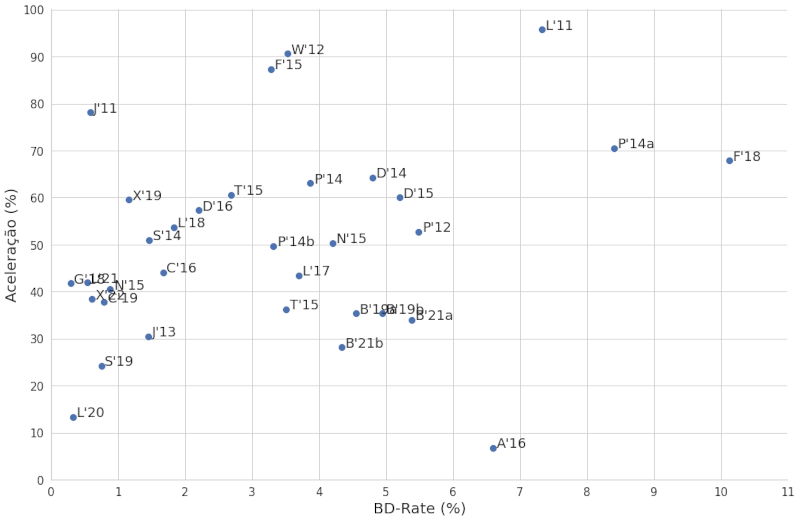
\includegraphics[width=0.8\linewidth]{FIGURES/fig_12.png}
    \caption{Valores de redução do tempo e do impacto na eficiência de codificação dos trabalhos selecionados pela revisão sistemática da literatura. Fonte: Elaborada pelo autor.}
    \label{fig:12}
\end{figure}
\end{landscape}
}


Uma análise mais aprofundada dos artigos apresentados na Tabela \ref{tab:III} permite observar que a reutilização do particionamento de blocos é a estratégia preferida para acelerar o processo de transcodificação, principalmente após o ano de 2015. Isso pode ser explicado porque o particionamento de blocos é uma tarefa essencial na codificação de vídeo, representando o principal laço de repetição do complexo processo de Otimização Taxa-Distorção (do inglês, \textit{Rate-Distortion Optimization}, RDO) \cite{bib:rdo_sullivan}, com decisões que afetam todos os estágios de codificação, direta ou indiretamente. A seção \ref{cap:3.3} cobre com mais detalhes essa categoria de soluções.

Por fim, é perceptível que a perda de eficiência de compressão diminuiu significativamente nos trabalhos publicados nos últimos anos. De fato, 70\% dos artigos da Tabela \ref{tab:III} que atingem um BD-rate inferior a 3\% empregam soluções baseadas em aprendizado de máquina para acelerar as decisões de transcodificação. Por essa razão, discutimos essa categoria de forma mais minuciosa na seção \ref{cap:3.2}.
